%--------------------------------------------------------------------------------
% 
\chapter{Evaluation}
%--------------------------------------------------------------------------------
Validation of the proposed approach was performed using our Curious Cat system 
running alive over the course of 4 years engaging a total of 728 registered 
users. During that time, the users checked-into 5,551 locations and responded 
to 57,978 questions, of which 8,611 were voting questions (7,560 positive and 
1,051 negative votes), 18,907 answered with "I dont know", and 30,460 real 
answers inserted into the KB as new knowledge, including 31,140 concepts 
(3,171 on users, 22,563 check-ins and other places and 5,406 other concepts). 
These triggered additional 386,980 assertions to be added through 
forward-chained inference. These can be separated into facts (374,300 
assertions) and additional derived question generating rules and questions 
(12,680). Altogether we gathered 444,958 (374,300 + 30,460) pieces of 
completely new knowledge. 

For easier understanding, we show the structure of the collected knowledge 
graphically in \autoref{fig:results}, and give real examples of the collected 
and inferred knowledge in \autoref{tab:results}.

\begin{figure}[h]
	\centering
		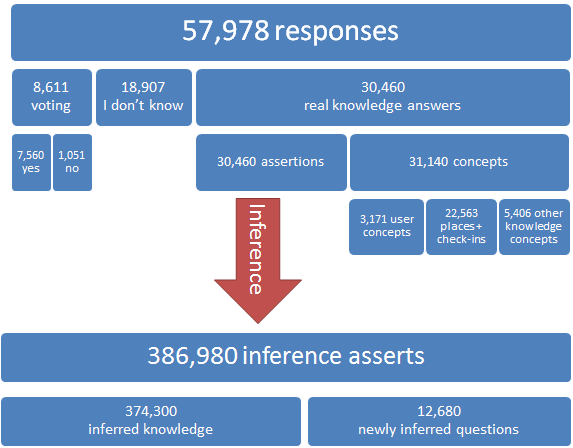
\includegraphics[width=1\textwidth]{figures/results.png}
	\caption{Graphical representation of collected answers (knowledge) and 
    distributions.}
	\label{fig:results}
\end{figure}

\begin{table}[h]
\centering
\caption{Examples of answered/asserted and inferred knowledge taken from
\emph{Curious Cat} KB.}
\label{tab:ccresultexamples}
\begin{tabular}{|c|l|l|}
	\hline
	\makecell[l]{\textbf{Type of the} \\ \textbf{collected knowledge}} & \textbf{Curious Cat Question} & \textbf{User Answer} \\
    \hline
    \textbf{User Concepts} &\makecell[l]{[automatic assert \\from registration]} & \makecell[l]{$is(User1,Person)$, \\ $name(User1,"Luka")$} \\
    \hline
    \textbf{Places + Check-ins} &\makecell[l]{[automatic assert \\from check-in \\ and Foursquare/\\Factual locations]} & \makecell[l]{$is(Place1,Restaurant)$, \\ $name(Place1,$\\"Pig'n Whistle"$)$} \\
     \hline
    \textbf{Other Concepts} &\makecell[l]{What did you order?} & \makecell[l]{Duck meat} \\
	\hline 
    \textbf{Real Knowledge 1} & Who is CEO of BMW? & Harald Kruger\\
	\hline
    \textbf{Real Knowledge 2} &\makecell[l]{What is the ticker symbol\\ of BMW?} & ABC \\
	\hline
    \textbf{voting(yes)} &\makecell[l]{Is it true that Herald Krueger\\ is the CEO of BMW company?} & yes \\
	\hline
    \textbf{voting(no)} &\makecell[l]{Is it true that ABC \\is the ticker symbol for BMW?} & no \\
	\hline
    \textbf{I don't know} &\makecell[l]{\_\_\_ and BMW are \\corporate competitors.} & I don't know \\
	\hline
    \textbf{Inferred knowledge 1} &\multicolumn{2}{l|}{$is(HeraldKrueger,Person)$} \\
	\hline
    \textbf{Inferred knowledge 2} &\multicolumn{2}{l|}{$anatomicalParts(HeraldKrueger,Hand)$} \\
	\hline
    \makecell[l]{\bfseries{Newly Inferred}\\ \bfseries{question}} &\multicolumn{2}{l|}{"What is Herald Krueger's age?"} \\
	\hline
\end{tabular}
\end{table}

While the resulting number and quality (\hl{Table XI, Table XII}) of assertions
shows that the presented approach can be successfully used for high quality KA,
we explored in more detail the contributions of specific characteristics of our
system and compare them to the baselines, to evaluate the ideas and claims
of the approach:
\begin{enumerate}
\item Using context to proactively drive the KA increases engagement and the 
chance of getting an answer (\hl{ref old 5.1})
\item Pre-existing knowledge and automated inference can be used to filter-out 
inconsistent answers and thus increase the quality of the acquired knowledge
\item Using newly acquired knowledge to further drive the KA process increases the amount of acquired answers and reach of the system
\item Crowdsourcing additionally improves the results by filtering wrong but logically correct answers
\end{enumerate}

\section{Context and Proactivity}
\label{section:evaluationContext}
\emph{Curious Cat} employs two contextual knowledge provision mechanisms. One 
is location based knowledge, such as, the type of current location, the time of
visit and the duration of stay. The second is internal knowledge that the 
system already knows about the user, such us, languages that the user speaks, 
food she likes, demographics data, interests, etc. In evaluation, we focused on
exploring benefits of using the location based context, since it is practically
impossible to disable internal knowledge without bigger changes in the system. 
Inferring without internal knowledge e.g., total removal of the personal 
knowledge would mean removal of almost all questions regarding people, animals,
human interests, etc., since these are general for human beings and to some 
extent to animals as well.

For the purpose of this experiment, we deliberately removed GPS location and 
connected mechanisms for derived knowledge for a duration of three months. We 
normalized the measures (assertions per user per day) for all experiments to 
level out the differences in the durations of experiments against a longer 
duration of fully operative system. The results are presented in 
\autoref{tab:ccresultscompare}. The columns in the table are organized as 
follows:

\begin{itemize}
\item first column contains measure name,
\item second column full data-set when using context (marked as C),
\item third is 100-day data-set when not using context (NC100),
\item and last is the normalized column with context (C100) which makes it 
possible to compare the context versus no context knowledge collection behavior (C100 vs NC100).
\end{itemize}

Since number of days and users is strongly correlated with the number of 
answers the system gets, and we only have the "No Context" data for 100 days 
(41 new users during that time and 45 active users), we normalized our 
"Context data" in such a way, that it matches the duration, new users and 
active users of \emph{NC100}. For this, we had to scan all the data-set 
day-by day with a range of 100-day window, where we looked at the number of new 
and active users in each of the 1264 sub-windows (number of all different 
100 day windows one can fit into 1264 days). In the whole data-set there was 
18 such 100-day windows, which can be directly compared to the \emph{NC100}. 
While the number of new users is fixed to 41, number of new assertions and 
active users still varies (min. 1,429, max. 9,279 new assertions and min. 47, 
max 61 active users). For this reason, we calculated the mean values of all 
18 windows which had the same number of new users as \emph{NC100}. Matching 
new users (instead of active users) was selected because new users are the
ones that contribute most of the assertions, since their interest winds down 
gradually. This can be seen on \hl{old Fig. 13}. This is also the primary 
reason why (unintuitively) number of new assertions/day/active user 
(row 7 in {utoref{tab:ccresultscompare}) is higher without context 
(\emph{NC100}) than for  non-normalized data from experiment using context 
(\emph{C}).

\begin{table}[h]
\centering
\caption{Results of KA without context versus results while using location based context}
\label{tab:ccresultscompare}
\begin{tabular}{|l|l|l|l|}
	\hline
	\textbf{Measure}  & \makecell[l]{\textbf{With Location}\\\textbf{Context (C)}} & \makecell[l]{\textbf{Without Location}\\ \textbf{Context (NC100)}} &  \makecell[l]{\textbf{With Location}\\\textbf{Context 100}\\\textbf{days (C100)}}\\
    \hline
    1. Experiment duration & 1,364 days & 100 days & 100 days \\
    \hline
    2. Number of new assertions & 56,586 & 709 & 2,244 (+216.5\%) \\
    \hline
    \makecell[l]{3. Number of new assertions\\where user didn't\\ know the answer} & 18,380 (32\%) & 267 (38\%) & 667 (28.3\% = -9.7\%) \\
	\hline 
    \makecell[l]{4. Number of new \\assertions where \\user knew the answer}  &38,206 (68\%) & 442 (62\%) & 1,577 (71.7\% = +9.7\%) \\
	\hline
    \makecell[l]{5. Number of new \\assertions/day \\(all users) } & 42.1 & 7.1 & 22.4 (+215.5\%)\\
	\hline
    \makecell[l]{6. Number of new \\assertions/active user } & 90.3 & 15.7 & 44.2 (+181.5\%) \\
	\hline
    \makecell[l]{\textbf{7. Number of new}\\\textbf{assertions/day/active}\\\textbf{user}} & 0.07 & 0.16 & \textbf{0.44 (+175\%)} \\
	\hline
    \makecell[l]{8. Number of new \\concepts/day} & 3.7 & 0.4 & 2.4 (+85.2\%) \\
	\hline
    \makecell[l]{9. Number of new concepts \\ (excluding users and\\ locations)} & 4,925 & 36 & 243 (+85.2\%) \\
	\hline
    10. Number of active users & 625 & 45 & 49 \\
	\hline
    11. Number of new users & 625 & 41 & 41 \\
	\hline
\end{tabular}
\end{table}

The results of not using context show the decrease of raw new knowledge 
assertions from 56,568 to 709, which of course can be attributed to the fact 
that duration of experiment \emph{C} was much longer, or that it had more users
than \emph{NC100}. As described above, this is properly normalized in the 
column \emph{C100}, where the raw number of assertions raises to 2,244 
compared to only 709 when not using context (\textbf{context brings 217\% 
increase}).

While the majority of the increase is due to pro-active questions from 
\emph{Curious Cat}, which are linked to GPS clustering, some of the increase 
is also due to better targeting of the questions due to contextual data, 
since without the context only users are selecting the topics and the system 
doesnt have enough knowledge to successfully pick the most relevant next 
question. This is reflected in a slight increase in the proportion of the 
questions for which the user knows the answer (+9.7\% - row 4 in 
\autoref{tab:ccresultscompare}). This is independently of pro-active component 
which is mostly reflected in the raw number of assertions, while the 
knowing/not knowing ratio improvement is due to better targeting whatever 
question there was.

%subsection
\subsection{Consistency Checking}
\label{section:resultsConsistencyChecking}
Before the system accepts the answer from the user (as described in 
\hl{old section 4.6}), it converts it into logic and checks whether it is 
consistent with its current knowledge. If there is an inconsistency, it will 
reject the answer and thus prevent the wrong or contradicting knowledge to 
corrupt the KB and consequently the future KA process. The user then either has
to fix the answer, or convince the system that the answer is actually only a 
different name for the consistent knowledge. For example, if the user states 
that he ate a car in the restaurant, this is either wrong, or car is the name 
for some unknown food and not a vehicle.

Due to development process and timeline of the system, we only have logs and 
consequently insights on when/how the system rejected the answers due to 
inconsistency for 143 out of 1,472 days of the experiment duration. During 
this time, 148 users provided 23,543 answers and the system rejected 563 of 
them, so 22,980 of assertions went into the KB. Among the 563 rejections, 
some of them were repeating (user re-tries, or other users did the same 
mistake), so the system actually prevented 384 unique inconsistent answers.

%old table VII

\begin{table}[h]
\centering
\caption{Results of Consistency Checking}
\label{tab:resultsconsistencycheck}
\begin{tabular}{|l||l|l|}
	\hline
	\textbf{Measure}  &	 \makecell[l]{\textbf{Real data from}\\\textbf{the logs}} & \makecell[l]{\textbf{Extrapolation for}\\ \textbf{the full experiment}} \\
    \hline
    Number of new assertions & 1,364 days & 100 days \\
    \hline
    \makecell[l]{Number of rejected assertions\\due to inconsistency} & 56,586 & 709\\
    \hline
    \makecell[l]{\textbf{Percentage of rejected}\\\textbf{asserts}} & 18,380 (32\%) & 267 (38\%) \\	
	\hline 
    \makecell[l]{Number of unique rejected\\ asserts}  &38,206 (68\%) & 442 (62\%) \\
	\hline
    \makecell[l]{\textbf{Percentage of unique}\\ \textbf{rejected asserts}} & 42.1 & 7.1\\
	\hline
    \makecell[l]{Number of new users } & 90.3 & 15.7 \\
	\hline
    \makecell[l]{Number of active users} & 0.07 & 0.16 \\
	\hline
    \makecell[l]{Experiment duration} & 3.7 & 0.4 \\
	\hline
\end{tabular}
\end{table}


